%+TITLE: Rotaciones en 2D
%+DESCRIPTION: Como preludio al estudio de los grupos consideramos las rotaciones.
\documentclass[11pt,a4paper]{article}

\usepackage[utf8]{inputenc}
\usepackage[T1]{fontenc}
\usepackage[spanish,es-nodecimaldot]{babel}
\usepackage{lmodern}
\usepackage{amsmath,amssymb,mathtools}
\usepackage{graphicx}
\usepackage{xcolor}
\usepackage{geometry}
\usepackage{enumitem}
\usepackage{microtype}

\geometry{margin=2.3cm}
\setlength{\parindent}{0pt}
\setlength{\parskip}{0.65em}
\setlist[itemize]{leftmargin=1.6em,itemsep=0.25em,topsep=0.25em}

\definecolor{title-red}{RGB}{165,25,20}
\definecolor{concept-green}{RGB}{20,125,45}
\newcommand{\concept}[1]{\textcolor{concept-green}{#1}}

\newcommand{\ket}[1]{\left|#1\right\rangle}
\newcommand{\bra}[1]{\left\langle#1\right|}
\newcommand{\braket}[2]{\left\langle #1\middle|#2\right\rangle}
\newcommand{\hc}{\mathrm{h.c.}}
\newcommand{\Tr}{\operatorname{Tr}}
\newcommand{\Diffs}{\mathrm{Diffs}}

\begin{document}

Para empezar a explorar las simetrías, estudiemos una de las más sencillas: las rotaciones en 2 dimensiones. Para esto, consideremos un punto en el plano con coordenadas $(x,y)$ y hagamos una rotación por un ángulo $\theta$.

\begin{figure}
  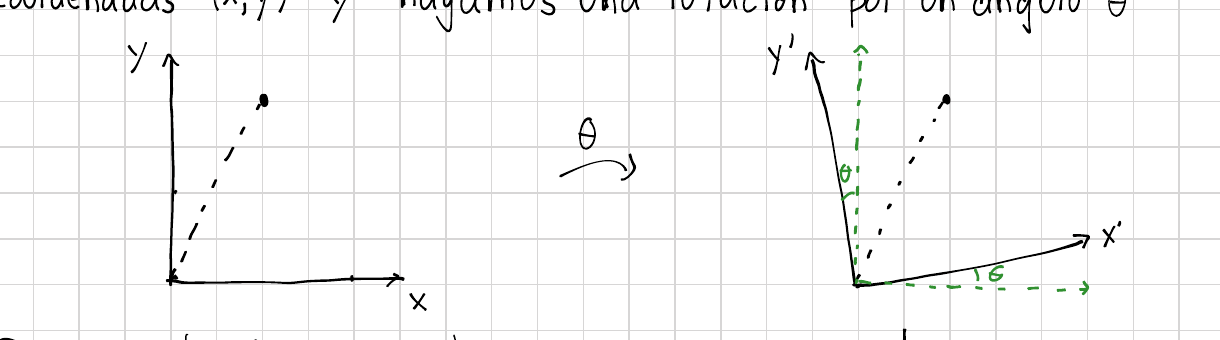
\includegraphics[width=0.78\textwidth]{figures/rotacion_general_2d.png}
\end{figure}

Para ver la forma que tienen $x'$ y $y'$, consideremos primero un punto en el eje $\hat x$. Al rotarlo tenemos
\[
  x'=x\cos\theta,
  \qquad
  y'=-x\sen\theta.
\]

\begin{center}
  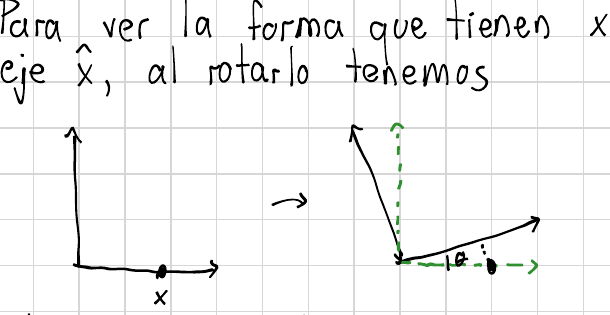
\includegraphics[width=0.42\textwidth]{figures/rotacion_eje_x.png}
\end{center}

Ahora hagamos lo mismo para un punto sobre el eje $\hat y$:
\[
  x'=y\sen\theta,
  \qquad
  y'=y\cos\theta.
\]

\begin{figure}
  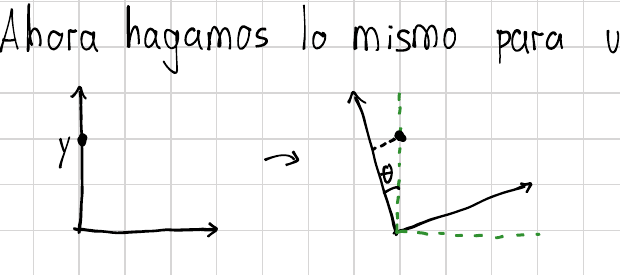
\includegraphics[width=0.42\textwidth]{figures/rotacion_eje_y.png}
\end{figure}

Como cualquier punto se puede escribir como una combinación lineal de los vectores $\hat i=(1,0)$ y $\hat j=(0,1)$, podemos calcular la rotación de cualquier vector.

En el sistema $(x',y')$, tenemos
\[
  \hat i=(\cos\theta,-\sen\theta),
  \qquad
  \hat j=(\sen\theta,\cos\theta),
\]
es decir,
\[
  \hat i=\cos\theta\,\hat i'-\sen\theta\,\hat j',
  \qquad
  \hat j=\sen\theta\,\hat i'+\cos\theta\,\hat j'.
\]

Ahora tomemos un vector arbitrario:
\begin{align*}
  \vec v
  &=v_x\hat i+v_y\hat j \\
  &=\left(v_x\cos\theta+v_y\sen\theta\right)\hat i'
   +\left(v_y\cos\theta-v_x\sen\theta\right)\hat j'.
\end{align*}

En otras palabras,
\[
  v_x'=v_x\cos\theta+v_y\sen\theta,
  \qquad
  v_y'=v_y\cos\theta-v_x\sen\theta.
\]

Esto también lo podemos escribir en notación matricial:
\[
  \begin{pmatrix}
    v_x'\\ v_y'
  \end{pmatrix}
  =
  \begin{pmatrix}
    v_x\cos\theta+v_y\sen\theta\\
    v_y\cos\theta-v_x\sen\theta
  \end{pmatrix}
  =
  \underbrace{
  \begin{pmatrix}
    \cos\theta & \sen\theta\\
    -\sen\theta & \cos\theta
  \end{pmatrix}}_{\text{matriz de rotación }R_\theta}
  \begin{pmatrix}
    v_x\\ v_y
  \end{pmatrix}.
\]

Notemos que
\begin{align*}
  R^TR
  &=
  \begin{pmatrix}
    \cos\theta & -\sen\theta\\
    \sen\theta & \cos\theta
  \end{pmatrix}
  \begin{pmatrix}
    \cos\theta & \sen\theta\\
    -\sen\theta & \cos\theta
  \end{pmatrix} \\
  &=
  \begin{pmatrix}
    \cos^2\theta+\sen^2\theta & 0\\
    0 & \cos^2\theta+\sen^2\theta
  \end{pmatrix}
  =
  \begin{pmatrix}
    1&0\\0&1
  \end{pmatrix}.
\end{align*}

Estas matrices son ortogonales. Además preservan el módulo de los vectores:
\[
  v_x'^2+v_y'^2
  =v_x^2(\cos^2\theta+\sen^2\theta)
   +v_y^2(\cos^2\theta+\sen^2\theta)
  =v_x^2+v_y^2.
\]

De hecho esto último es cierto para cualquier matriz ortogonal. Si tenemos $\vec v'=R\vec v$, entonces
\[
  \vec v'{}^T\vec v'
  =(R\vec v)^T(R\vec v)
  =\vec v^{\,T}R^TR\vec v
  =\vec v^{\,T}\vec v.
\]

De hecho las matrices $R_\theta$ son las matrices de rotación más generales. (Tarea.)

Las rotaciones forman un grupo:
\begin{align*}
  R_{\theta_1}R_{\theta_2}
  &=
  \begin{pmatrix}
    \cos\theta_1 & \sen\theta_1\\
    -\sen\theta_1 & \cos\theta_1
  \end{pmatrix}
  \begin{pmatrix}
    \cos\theta_2 & \sen\theta_2\\
    -\sen\theta_2 & \cos\theta_2
  \end{pmatrix} \\
  &=
  \begin{pmatrix}
    \cos\theta_1\cos\theta_2-\sen\theta_1\sen\theta_2
      & \sen\theta_1\cos\theta_2+\sen\theta_2\cos\theta_1\\
    -\sen\theta_1\cos\theta_2-\sen\theta_2\cos\theta_1
      & \cos\theta_1\cos\theta_2-\sen\theta_1\sen\theta_2
  \end{pmatrix} \\
  &=R_{\theta_1+\theta_2},
\end{align*}
que es una rotación.

También,
\begin{align*}
  (R_{\theta_1}R_{\theta_2})^T(R_{\theta_1}R_{\theta_2})
  &=R_{\theta_2}^TR_{\theta_1}^TR_{\theta_1}R_{\theta_2}
   =R_{\theta_2}^TR_{\theta_2}
   =\mathbb{1}.
\end{align*}

La multiplicación de matrices es asociativa, así como la multiplicación por un escalar.

Además,
\[
  R_\theta R_{-\theta}=R_0=\mathbb{1},
\]
por lo que existe la inversa.

Es también un grupo que depende de un parámetro continuo, el ángulo. De hecho podemos escribir una rotación infinitesimal como
\[
  R_\epsilon
  =
  \begin{pmatrix}
    \cos\epsilon&\sen\epsilon\\
    -\sen\epsilon&\cos\epsilon
  \end{pmatrix}
  \approx
  \begin{pmatrix}
    1&\epsilon\\
    -\epsilon&1
  \end{pmatrix}
  =\mathbb{1}+i\epsilon
  \underbrace{
  \begin{pmatrix}
    0&-i\\ i&0
  \end{pmatrix}}_{\text{generador de la rotación }J}.
\]

De hecho cualquier rotación se puede escribir como
\[
  R_\theta=e^{i\theta J}.
\]

Note que $J^2=\mathbb{1}$. Esto implica
\[
  J^{2n}=(J^2)^n=\mathbb{1},
  \qquad
  J^{2n+1}=J^{2n}J=J.
\]
Por tanto,
\begin{align*}
  e^{i\theta J}
  &=\sum_{n=0}^\infty\frac{1}{n!}(i\theta)^nJ^n \\
  &=\sum_{n=0}^\infty\frac{1}{(2n)!}(-1)^n\theta^{2n}J^{2n}
   +i\sum_{n=0}^\infty\frac{1}{(2n+1)!}(-1)^n\theta^{2n+1}J^{2n+1} \\
  &=\cos\theta\,\mathbb{1}+i\sen\theta\,J \\
  &=
  \begin{pmatrix}
    \cos\theta&0\\0&\cos\theta
  \end{pmatrix}
  +
  \begin{pmatrix}
    0&\sen\theta\\-\sen\theta&0
  \end{pmatrix}
  =R_\theta.
\end{align*}

Este grupo se llama $O(2)$.

Un grupo similar es el de los complejos unimodulares $|z|=1$, llamado $U(1)$:
\[
  |z_1z_2|=|z_1||z_2|=1,
  \qquad |1|=1,
  \qquad |z^{-1}|=\frac1{|z|}=1,
  \qquad \text{etc.}
\]

\begin{center}
  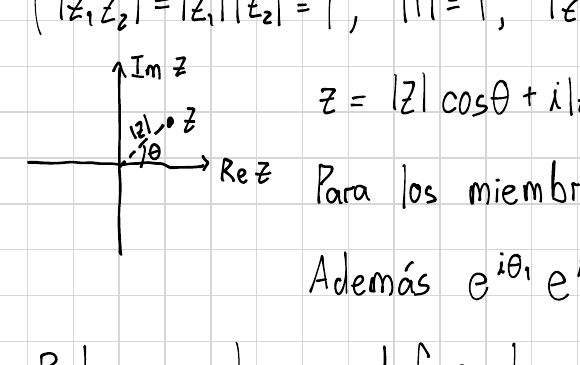
\includegraphics[width=0.30\textwidth]{figures/plano_complejo_u1.png}
\end{center}

En general,
\[
  z=|z|\cos\theta+i|z|\sen\theta=|z|e^{i\theta}.
\]
Para los miembros de $U(1)$,
\[
  z=e^{i\theta},
\]
y además
\[
  e^{i\theta_1}e^{i\theta_2}=e^{i(\theta_1+\theta_2)}.
\]

Podemos entonces definir la correspondencia
\[
  R_\theta\longrightarrow e^{i\theta}.
\]
Llamémosla
\[
  f(R_\theta)=e^{i\theta}.
\]
Note que $f$ es biyectiva: a cada $R_\theta$ le corresponde uno y sólo un $e^{i\theta}$.

Además,
\[
  f(R_{\theta_1}R_{\theta_2})
  =f(R_{\theta_1+\theta_2})
  =e^{i(\theta_1+\theta_2)}
  =e^{i\theta_1}e^{i\theta_2}.
\]
Es decir, es un \concept{homomorfismo}.

Un homomorfismo es un mapa que preserva la estructura. Cuando es biyectivo, lo llamamos \concept{isomorfismo}. Dos grupos isomorfos contienen la misma información y estructura. Los interpretamos como el ``mismo'':
\[
  O(2)\simeq U(1).
\]
\end{document}
